\documentclass[aspectratio=169,10pt]{beamer}
\usepackage{hud_theme}

\hypersetup{
  pdftitle={Wizard's Chess — Alpha-Beta vs MCTS | HW2},
  pdfauthor={Group 7 · CC01 · HCMUT},
  pdfsubject={Introduction to Artificial Intelligence (CO3061)},
  colorlinks=true,
  linkcolor=HudLavender,
  urlcolor=HudTeal
}

\begin{document}

% ======================================================================
% SLIDE 01 — COVER
% ======================================================================
\begingroup
\setbeamertemplate{background canvas}{%
  \begin{tikzpicture}[x=1cm,y=1cm]
    \useasboundingbox (0,0) rectangle (16,9);
    \fill[HudBg] (0,0) rectangle (16,9);

    % Right 55% Panel: Wizard's Chess 3D Board with smooth cinematic vignette
    \begin{scope}
      \clip (7.10,0) rectangle (16,9);
      \fill[HudBgDeep] (7.10,0) rectangle (16,9);
      \node[anchor=center, inner sep=0pt] at (11.55,4.72)
        {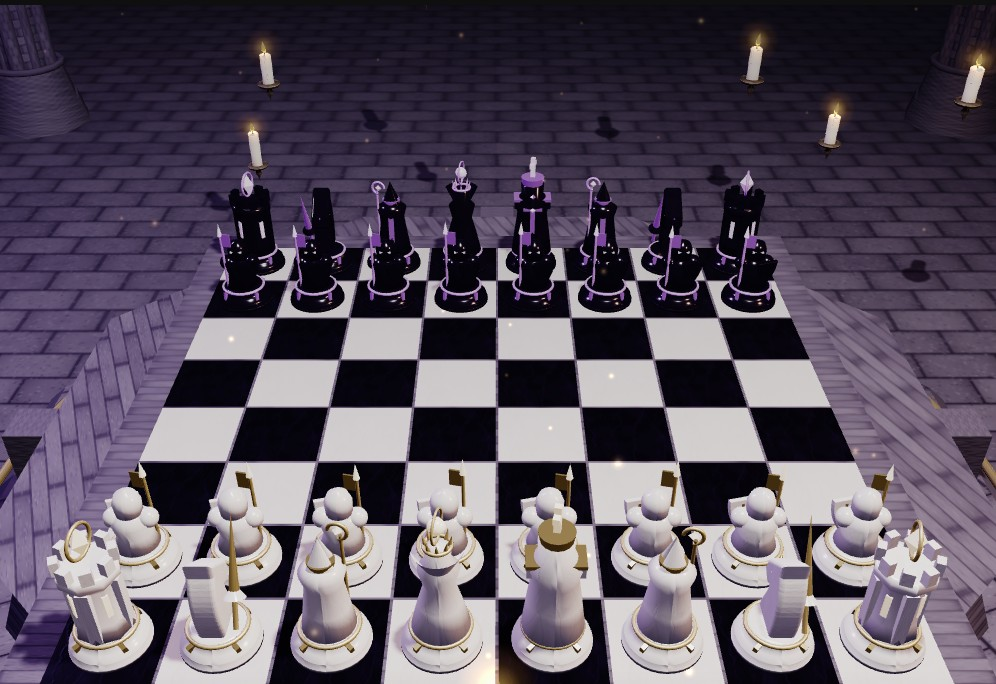
\includegraphics[width=9.25cm]{images/hud_cover.jpg}};
      % Left feather into #0F0C14
      \fill[HudBg, opacity=0.95] (7.10,0) rectangle (7.38,9);
      \fill[HudBg, opacity=0.72] (7.38,0) rectangle (7.66,9);
      \fill[HudBg, opacity=0.42] (7.66,0) rectangle (7.96,9);
      \fill[HudBg, opacity=0.18] (7.96,0) rectangle (8.30,9);
      % Top & bottom soft vignette blends into HudBg (low bottom bands preserve white piece bases)
      \fill[HudBg, opacity=0.95] (7.10,7.75) rectangle (16,9);
      \fill[HudBg, opacity=0.65] (7.10,7.38) rectangle (16,7.75);
      \fill[HudBg, opacity=0.30] (7.10,7.00) rectangle (16,7.38);
      \fill[HudBg, opacity=0.95] (7.10,0) rectangle (16,0.90);
      \fill[HudBg, opacity=0.55] (7.10,0.90) rectangle (16,1.25);
      \fill[HudBg, opacity=0.22] (7.10,1.25) rectangle (16,1.58);
    \end{scope}

    % Cover HUD Corner Brackets
    \draw[HudBorder!70, line width=0.95pt] (0.28,8.28) -- (0.28,8.72) -- (0.72,8.72);
    \draw[HudBorder!70, line width=0.95pt] (15.28,8.72) -- (15.72,8.72) -- (15.72,8.28);
    \draw[HudBorder!70, line width=0.95pt] (0.28,0.72) -- (0.28,0.28) -- (0.72,0.28);
    \draw[HudBorder!70, line width=0.95pt] (15.28,0.28) -- (15.72,0.28) -- (15.72,0.72);
    \fill[HudLavender] (0.28,8.72) circle (0.04) (15.72,8.72) circle (0.04)
                       (0.28,0.28) circle (0.04) (15.72,0.28) circle (0.04);

    % Top-right 4-chip indicator (chip 1 active)
    \node[anchor=east, fill=HudPanel, opacity=0.90, draw=HudBorder!45,
          rounded corners=3pt, inner xsep=6pt, inner ysep=3pt] at (15.15,8.44) {%
      \tikz[x=1cm,y=1cm]{
        \fill[HudLavender, rounded corners=1.2pt] (0,0) rectangle (0.20,0.20);
        \fill[HudTrack, rounded corners=1.2pt] (0.30,0) rectangle (0.50,0.20);
        \fill[HudTrack, rounded corners=1.2pt] (0.60,0) rectangle (0.80,0.20);
        \fill[HudTrack, rounded corners=1.2pt] (0.90,0) rectangle (1.10,0.20);
      }%
    };

    % Top-left HCMUT lockup
    \node[anchor=west, inner sep=0pt] (bk) at (0.85,8.05) {
\includegraphics[height=0.68cm]{images/BK.png}};
    \node[anchor=west, inner sep=0pt, align=left] at (1.72,8.05) {%
      {\fontsize{7.5}{9}\selectfont\bfseries\color{HudIvory}HCMUT $\cdot$ VNU-HCM}\\[2pt]
      {\fontsize{6.8}{8.5}\selectfont\color{HudMuted}Faculty of Computer Science \& Engineering}%
    };

    % Eyebrow pill
    \node[anchor=west, inner sep=0pt] at (0.85,6.88) {\hudtag[HudLavender]{GROUP 7 $\cdot$ CC01 $\cdot$ CO3061 $\cdot$ HW2}};

    % Main Gold Cinzel Title + Subtitle
    \node[anchor=west, inner sep=0pt, align=left] at (0.82,5.42) {%
      {\huddisplay\fontsize{28}{31}\selectfont\color{HudGold}WIZARD'S}\\
      {\huddisplay\fontsize{28}{31}\selectfont\color{HudGold}CHESS}\\[4pt]
      {\huddisplay\fontsize{10.5}{13}\selectfont\color{HudGold}ALPHA-BETA VS MCTS}%
    };

    % Diamond divider
    \node[anchor=west, inner sep=0pt] at (0.85,3.82) {\huddivider{4.8}};

    % Lavender tagline
    \node[anchor=west, inner sep=0pt, align=left] at (0.85,3.12) {%
      {\fontsize{11.5}{15}\selectfont\color{HudLavender}Two search strategies.}\\
      {\fontsize{11.5}{15}\selectfont\color{HudLavender}One chessboard.}%
    };

    % Metadata block (Inter for clean Vietnamese rendering)
    \node[anchor=west, inner sep=0pt, align=left] at (0.85,1.62) {%
      {\fontsize{8.2}{11.5}\selectfont\color{HudMuted}Course: \color{HudIvory}Introduction to Artificial Intelligence (CO3061)}\\
      {\fontsize{8.2}{11.5}\selectfont\color{HudMuted}Advisor: \color{HudIvory}Dr. Nguyễn Quốc Minh}%
    };

    % Cover bottom footer
    \draw[HudBorder!45, line width=0.5pt] (0.85,0.68) -- (6.80,0.68);
    \node[anchor=west, inner sep=0pt, font=\ttfamily\fontsize{6.5}{7.5}\selectfont, text=HudMuted]
      at (0.85,0.42) {WIZARD'S CHESS \ / \ INTRO AI \ $\cdot$ \ HCMUT};
    \node[anchor=east, inner sep=0pt, font=\ttfamily\bfseries\fontsize{8}{9}\selectfont, text=HudLavender]
      at (15.15,0.42) {01};
  \end{tikzpicture}%
}
\begin{frame}[plain]
\mbox{}
\end{frame}
\endgroup

% ======================================================================
% SECTION 01 — THE PROBLEM (Slides 02–03)
% ======================================================================
\hudsetsection{1}{01 / THE PROBLEM}
\hudgridon

% SLIDE 02 — CHESS AS A SEARCH PROBLEM
\begin{frame}{CHESS AS A SEARCH PROBLEM}
\framesubtitle{Choose a move while accounting for the opponent's strongest reply}
\vspace{0.10cm}
\begin{columns}[T,onlytextwidth]
  \begin{column}{5.3cm}
    \hudhero[HudLavender]{40}{\raisebox{0.12ex}{\textsf{\fontsize{28}{28}\selectfont$\sim$}}35}\par
    \vspace{3pt}
    {\fontsize{10.5}{13}\selectfont\bfseries\color{HudGold}CHOICES AT EACH PLY}\par
    \vspace{6pt}
    {\fontsize{9.2}{13}\selectfont\color{HudIvory}A move is only as good as the opponent's strongest reply allows.}\par
    \vspace{8pt}
    \hudtag[HudTeal]{EBF $\approx$ 35.0 (PLAIN MINIMAX)}\par
    \vspace{8pt}
    \hudcardaccent[6pt]{HudBorder}{4.7cm}{%
      {\fontsize{8}{11.2}\selectfont\color{HudMuted}%
        $\bullet$ \textbf{\color{HudIvory}1 ply} = one move by one side\\
        $\bullet$ At depth 4, Minimax expands \textbf{\color{HudLavender}1.5M nodes}\\
        $\bullet$ Exhaustive search is impractical
      }%
    }
  \end{column}
  \begin{column}{8.6cm}
    \hudcard{7.85cm}{%
      \centering
      \begin{tikzpicture}[x=0.98cm,y=0.98cm]
        \tikzstyle{pnode}=[fill=HudTrack, draw=HudLavender!80, line width=0.8pt,
                           rounded corners=8pt, minimum width=1.60cm, minimum height=0.50cm,
                           font=\fontsize{8}{9}\selectfont\bfseries, text=HudIvory]
        \tikzstyle{lnode}=[fill=HudPanelAlt, draw=HudBorder!75, line width=0.7pt,
                           rounded corners=7pt, minimum width=1.18cm, minimum height=0.42cm,
                           font=\fontsize{7.5}{8.5}\selectfont, text=HudIvory]
        \tikzstyle{hnode}=[fill=HudPanel, draw=HudStone!55, dashed, line width=0.6pt,
                           rounded corners=7pt, minimum width=1.22cm, minimum height=0.42cm,
                           font=\ttfamily\fontsize{7}{8}\selectfont, text=HudMuted]

        \node[pnode, draw=HudGold] (root) at (3.7, 3.25) {Position};
        \node[pnode] (mA) at (1.75, 2.00) {Move A};
        \node[pnode] (mB) at (4.45, 2.00) {Move B};
        \node[hnode] (mDots) at (6.50, 2.00) {\dots\ ($\sim$35)};

        \node[lnode] (r1a) at (0.95, 0.72) {Reply 1};
        \node[lnode] (r2a) at (2.45, 0.72) {Reply 2};
        \node[lnode] (r1b) at (3.95, 0.72) {Reply 1};
        \node[lnode] (r2b) at (5.45, 0.72) {Reply 2};

        \draw[HudLavender!80, line width=0.85pt] (root) -- (mA) (root) -- (mB);
        \draw[HudStone!65, dashed, line width=0.7pt] (root) -- (mDots);
        \draw[HudBorder!80, line width=0.75pt] (mA) -- (r1a) (mA) -- (r2a)
                                             (mB) -- (r1b) (mB) -- (r2b);

        \node[font=\ttfamily\fontsize{7.2}{8.5}\selectfont, text=HudGold]
          at (3.7, 0.05) {STATE \ $\to$ \ ACTION \ $\to$ \ OPPONENT RESPONSE};
      \end{tikzpicture}
    }
  \end{column}
\end{columns}
\end{frame}

% SLIDE 03 — SHARED SEARCH ARCHITECTURE
\hudgridoff
\begin{frame}{SHARED SEARCH ARCHITECTURE}
\hudslidetag[HudLavender]{SHARED INTERFACE}
\framesubtitle{A common interface makes the algorithms directly comparable}
\vspace{0.10cm}

\noindent\begin{tikzpicture}[x=1cm,y=1cm]
  \useasboundingbox (0,0) rectangle (14.3,1.95);
  % 3 pipeline stage cards
  \node[fill=HudPanel, draw=HudBorder!45, rounded corners=5pt, inner sep=7.5pt,
        text width=3.65cm, minimum height=1.66cm, anchor=west, text=HudIvory] (c1) at (0,0.98) {%
    {\ttfamily\fontsize{7}{8}\selectfont\bfseries\color{HudGold}01 $\cdot$ INPUT}\\[4pt]
    {\fontsize{10.5}{13}\selectfont\bfseries\color{HudIvory}Position +}\\
    {\fontsize{10.5}{13}\selectfont\bfseries\color{HudIvory}search budget}\\[3pt]
    {\fontsize{7.4}{9.5}\selectfont\color{HudMuted}FEN / moves + time limit (1.0\,s)}%
  };
  \draw[HudLavender, line width=1.1pt, -{Stealth[length=2.2mm]}] (4.20,0.98) -- (4.90,0.98);

  \node[fill=HudPanelAlt, draw=HudLavender!65, line width=0.9pt, rounded corners=5pt, inner sep=7.5pt,
        text width=3.85cm, minimum height=1.66cm, anchor=west, text=HudIvory] (c2) at (4.98,0.98) {%
    {\ttfamily\fontsize{7}{8}\selectfont\bfseries\color{HudLavender}02 $\cdot$ SEARCH AGENT}\\[4pt]
    {\fontsize{10.5}{13}\selectfont\bfseries\color{HudIvory}Alpha-Beta}\\
    {\fontsize{10.5}{13}\selectfont\bfseries\color{HudIvory}or MCTS}\\[3pt]
    {\fontsize{7.4}{9.5}\selectfont\color{HudMuted}Unified \texttt{select\_move()} API}%
  };
  \draw[HudLavender, line width=1.1pt, -{Stealth[length=2.2mm]}] (9.38,0.98) -- (10.08,0.98);

  \node[fill=HudPanel, draw=HudBorder!45, rounded corners=5pt, inner sep=7.5pt,
        text width=3.58cm, minimum height=1.64cm, anchor=west, text=HudIvory] (c3) at (10.12,0.98) {%
    {\ttfamily\fontsize{7}{8}\selectfont\bfseries\color{HudTeal}03 $\cdot$ OUTPUT}\\[4pt]
    {\fontsize{10.5}{13}\selectfont\bfseries\color{HudIvory}Best move +}\\
    {\fontsize{10.5}{13}\selectfont\bfseries\color{HudIvory}statistics}\\[3pt]
    {\fontsize{7.4}{9.5}\selectfont\color{HudMuted}Depth, nodes, PV / visits}%
  };
\end{tikzpicture}\par

\vspace{0.10cm}
\noindent\huddivider{14.3}\par
\vspace{0.10cm}

\begin{columns}[T,onlytextwidth]
  \begin{column}{6.95cm}
    \hudcardaccent[7.5pt]{HudGold}{6.22cm}{%
      {\ttfamily\fontsize{7.2}{8.5}\selectfont\bfseries\color{HudGold}RULES \& MOVE GENERATION}\\[3pt]
      {\fontsize{8.3}{11.5}\selectfont\color{HudIvory}\texttt{python-chess} enforces board legality and move generation; all search engines, pruning, and evaluation are built from scratch.}%
    }
  \end{column}
  \begin{column}{6.95cm}
    \hudcardaccent[7.5pt]{HudLavender}{6.22cm}{%
      {\ttfamily\fontsize{7.2}{8.5}\selectfont\bfseries\color{HudLavender}CONTROLLED EVALUATION}\\[3pt]
      {\fontsize{8.3}{11.5}\selectfont\color{HudIvory}Alpha-Beta and MCTS-Eval share one handcrafted material + piece-square evaluator; MCTS-Random uses rollouts instead.}%
    }
  \end{column}
\end{columns}

\vspace{0.14cm}
{\centering\fontsize{7.8}{10}\selectfont\color{HudMuted}Experiments (E1--E5) and the Search Lab web API invoke the exact same agent interface.\par}
\end{frame}

% ======================================================================
% SECTION 02 — SEARCH METHODS (Slides 04–05)
% ======================================================================
\hudsetsection{2}{02 / SEARCH METHODS}
\hudgridon

% SLIDE 04 — ALPHA-BETA SEARCH
\begin{frame}{ALPHA-BETA SEARCH}
\hudslidetag[HudLavender]{MINIMAX + PRUNING}
\framesubtitle{Propagate the opponent's best response; prune branches that cannot change the decision}
\vspace{0.10cm}
\begin{columns}[T,onlytextwidth]
  \begin{column}{7.7cm}
    \hudcard{7.00cm}{%
      {\fontsize{8.3}{10}\selectfont\bfseries\color{HudLavender}A single refuting reply rules out a branch}\par
      \vspace{3pt}
      \centering
      \begin{tikzpicture}[x=0.98cm,y=0.98cm]
        \tikzstyle{tbox}=[fill=HudTrack, draw=HudLavender!80, line width=0.8pt,
                          rounded corners=7pt, minimum width=1.12cm, minimum height=0.42cm,
                          font=\fontsize{7.8}{9}\selectfont\bfseries, text=HudIvory]
        \node[tbox, draw=HudGold] (max) at (3.25, 2.95) {MAX};
        \node[tbox] (minL) at (1.50, 1.84) {MIN};
        \node[tbox] (minR) at (5.00, 1.84) {MIN};

        \node[tbox, minimum width=0.92cm] (l5) at (0.70, 0.70) {5};
        \node[tbox, minimum width=0.92cm] (l7) at (2.30, 0.70) {7};
        \node[tbox, minimum width=0.92cm, draw=HudGold] (l3) at (4.15, 0.70) {3};

        \draw[HudLavender!85, line width=0.9pt] (max) -- (minL) (max) -- (minR);
        \draw[HudLavender!85, line width=0.9pt] (minL) -- (l5) (minL) -- (l7) (minR) -- (l3);

        % Pruned branch + clean X mark
        \draw[HudGold!85, dashed, line width=0.95pt] (minR) -- (5.82, 0.82);
        \draw[HudCrimson, line width=1.5pt, line cap=round]
          (5.70,0.60) -- (6.00,0.90) (5.70,0.90) -- (6.00,0.60);

        % Bounds positioned in clean open whitespace with subtle badge backing
        \node[fill=HudPanel, inner sep=1.5pt, font=\ttfamily\fontsize{8}{9}\selectfont\bfseries, text=HudLavender]
          at (1.50, 1.24) {$\alpha = 5$};
        \node[fill=HudPanel, inner sep=1.5pt, font=\ttfamily\fontsize{8}{9}\selectfont\bfseries, text=HudGold]
          at (3.58, 1.34) {$\beta \le 3$};

        \node[anchor=west, font=\fontsize{7}{8.5}\selectfont, text=HudMuted]
          at (0.0, 0.08) {Illustrative values $\cdot$ fixed-depth minimax tree};
      \end{tikzpicture}
    }
  \end{column}
  \begin{column}{6.1cm}
    \hudcardaccent[8.5pt]{HudGold}{5.40cm}{%
      {\huddisplay\fontsize{15.5}{18}\selectfont\color{HudGold}PRUNE:\hspace{4pt}$3 \le 5$}\\[5pt]
      {\ttfamily\fontsize{7.8}{10}\selectfont\color{HudTeal}if alpha >= beta: prune remaining}\\[5pt]
      {\fontsize{8.3}{11.5}\selectfont\color{HudIvory}Once MIN finds $3$, its value is $\le 3$. MAX already guarantees $5$, so the sibling subtree is skipped.}%
    }\par
    \vspace{0.18cm}
    \hudcardaccent[8.5pt]{HudLavender}{5.40cm}{%
      {\ttfamily\fontsize{7.2}{8.5}\selectfont\bfseries\color{HudLavender}ENGINE ENHANCEMENTS}\\[5pt]
      {\fontsize{8.3}{12.5}\selectfont\color{HudIvory}%
        \hudcheck\ \ Iterative deepening\\
        \hudcheck\ \ Move ordering + transposition table\\
        \hudcheck\ \ Quiescence search at the horizon%
      }%
    }
  \end{column}
\end{columns}
\end{frame}

% SLIDE 05 — MONTE CARLO TREE SEARCH
\begin{frame}{MONTE CARLO TREE SEARCH}
\hudslidetag[HudGold]{SAMPLING + AVERAGES}
\framesubtitle{Explore promising lines while balancing exploration and exploitation}
\vspace{0.10cm}
\begin{columns}[T,onlytextwidth]
  \begin{column}{6.55cm}
    \hudcardaccent[5.5pt]{HudGold}{5.90cm}{%
      {\huddisplay\fontsize{11.5}{12.5}\selectfont\color{HudGold}01}\hspace{7pt}%
      \textbf{\color{HudIvory}Select} \ {\fontsize{7.8}{9.5}\selectfont\color{HudMuted}— UCT / PUCT balance}%
    }\par\vspace{4.5pt}
    \hudcardaccent[5.5pt]{HudGold}{5.90cm}{%
      {\huddisplay\fontsize{11.5}{12.5}\selectfont\color{HudGold}02}\hspace{7pt}%
      \textbf{\color{HudIvory}Expand} \ {\fontsize{7.8}{9.5}\selectfont\color{HudMuted}— Add candidate legal moves}%
    }\par\vspace{4.5pt}
    \hudcardaccent[5.5pt]{HudGold}{5.90cm}{%
      {\huddisplay\fontsize{11.5}{12.5}\selectfont\color{HudGold}03}\hspace{7pt}%
      \textbf{\color{HudIvory}Evaluate} \ {\fontsize{7.8}{9.5}\selectfont\color{HudMuted}— Rollout or heuristic leaf}%
    }\par\vspace{4.5pt}
    \hudcardaccent[5.5pt]{HudGold}{5.90cm}{%
      {\huddisplay\fontsize{11.5}{12.5}\selectfont\color{HudGold}04}\hspace{7pt}%
      \textbf{\color{HudIvory}Back up} \ {\fontsize{7.8}{9.5}\selectfont\color{HudMuted}— Update mean value + visits}%
    }\par\vspace{7pt}
    {\noindent\hudtag[HudMuted]{MCTS-Random}\hspace{1.5pt}\hudtag[HudGold]{MCTS-Eval}\hspace{1.5pt}\hudtag[HudGold]{Solver}\hspace{1.5pt}\hudtag[HudTeal]{Hybrid}}
  \end{column}
  \begin{column}{7.35cm}
    \hudcard{6.70cm}{%
      \centering
      \begin{tikzpicture}[x=0.95cm,y=0.95cm]
        \tikzstyle{mnode}=[fill=HudTrack, draw=HudLavender!75, line width=0.8pt,
                           rounded corners=7pt, minimum width=1.24cm, minimum height=0.42cm,
                           font=\fontsize{7.6}{9}\selectfont\bfseries, text=HudIvory]
        \tikzstyle{dot}=[fill=HudBorder!65, circle, inner sep=1.4pt]

        \node[mnode, draw=HudLavender] (root) at (3.25, 3.20) {Root};
        \node[mnode] (n12) at (1.00, 1.98) {$n = 12$};
        \node[mnode, draw=HudGold, line width=1pt] (n81) at (3.25, 1.98) {$n = 81$};
        \node[mnode] (n7) at (5.50, 1.98) {$n = 7$};
        \node[mnode, draw=HudGold, line width=1pt] (leaf) at (4.10, 0.72) {Leaf};

        % Terminated minor dots so no branches dangle into empty space
        \node[dot] (d1) at (0.55, 0.85) {};
        \node[dot] (d2) at (1.45, 0.85) {};
        \node[dot] (d3) at (2.55, 0.85) {};
        \node[dot] (d4) at (5.10, 0.85) {};
        \node[dot] (d5) at (5.90, 0.85) {};

        \draw[HudBorder!75, line width=0.7pt] (root) -- (n12) (root) -- (n7);
        \draw[HudBorder!55, line width=0.6pt] (n12) -- (d1) (n12) -- (d2)
                                             (n81) -- (d3) (n7) -- (d4) (n7) -- (d5);

        % Glowing high-visit path
        \draw[HudGold!35, line width=4.5pt] (root) -- (n81) -- (leaf);
        \draw[HudGold, line width=2.0pt] (root) -- (n81) -- (leaf);

        \node[font=\fontsize{7.4}{9}\selectfont\color{HudGold}]
          at (3.25, 0.08) {Thicker path = more visits \ $\cdot$ \ backup averages sampled leaves};
      \end{tikzpicture}
    }
  \end{column}
\end{columns}
\end{frame}

% ======================================================================
% SECTION 03 — EXPERIMENTAL EVIDENCE (Slides 06–09, ALL UNIFIED DARK HUD)
% ======================================================================
\hudsetsection{3}{03 / EXPERIMENTAL EVIDENCE}
\hudgridoff

% SLIDE 06 — EXPERIMENTAL DESIGN (Unified Dark Theme!)
\begin{frame}{EXPERIMENTAL DESIGN}
\hudslidetag[HudGold]{PROTOCOL $\cdot$ SEED 42}
\framesubtitle{Five controlled experiments connect playing strength to search behaviour}
\vspace{0.06cm}
\hudcard[inner sep=6pt]{13.55cm}{%
  \renewcommand{\arraystretch}{1.10}%
  \fontsize{8.0}{9.8}\selectfont
  \begin{tabular}{@{}>{\ttfamily\bfseries\color{HudGold}}p{0.85cm}>{\bfseries\color{HudIvory}}p{3.75cm}>{\color{HudLavender}}p{8.0cm}@{}}
    \toprule
    \textbf{\color{HudMuted}ID} & \textbf{\color{HudMuted}Experiment} & \textbf{\color{HudMuted}Question \& Primary Metric} \\
    \midrule
    E1 & Tournament strength & Round-robin score, W/D/L, relative Elo (7 agents, 1\,s/move) \\
    E2 & Budget scaling & Score vs time per move (AB vs MCTS-Eval, 0.05\,s -- 1.6\,s) \\
    E3 & Search efficiency & Mean nodes \& effective branching factor $b^*$ to depth 1--5 \\
    E4 & Verified tactics & Mate-in-1/2 solves \& trap-in-1/2 blunders (78 positions) \\
    E5 & Master agreement & Match rate \& chance-corrected $\kappa$ on 200 master positions \\
    \bottomrule
  \end{tabular}%
}\par
\vspace{0.10cm}
\hudcardaccent[5.5pt]{HudGold}{13.55cm}{%
  {\ttfamily\fontsize{7.6}{9.5}\selectfont\color{HudGold}E1 SETUP:}%
  \hspace{6pt}%
  {\fontsize{8.0}{10}\selectfont\color{HudIvory}1\,s per move $\cdot$ 4 openings $\times$ 2 colours = 8 games/pair $\cdot$ 168 games total $\cdot$ shared handcrafted evaluation}%
}
\end{frame}

% SLIDE 07 — ALPHA-BETA WON 48 / 48 GAMES
\begin{frame}{ALPHA-BETA WON 48 / 48 GAMES}
\hudslidetag[HudLavender]{E1 $\cdot$ TOURNAMENT $\cdot$ 1s/MOVE}
\framesubtitle{Tournament score $= (\mathrm{wins} + \tfrac{1}{2}\,\mathrm{draws}) / \mathrm{games}$ across 7 agents (48 games per agent)}
\vspace{0.10cm}
\begin{columns}[T,onlytextwidth]
  \begin{column}{4.85cm}
    \vspace{0.08cm}
    \hudhero[HudLavender]{46}{48}\par
    \vspace{3pt}
    {\fontsize{10}{12}\selectfont\bfseries\color{HudGold}WINS / 48 GAMES}\par
    \vspace{3pt}
    {\fontsize{9.2}{11.5}\selectfont\color{HudIvory}Every win by checkmate}\par
    \vspace{10pt}
    \hudcardaccent[6.5pt]{HudLavender}{4.3cm}{%
      {\fontsize{8}{11.2}\selectfont\color{HudMuted}%
        $\bullet$ \textbf{\color{HudIvory}95\% CI:} 93--100\%\\
        $\bullet$ \textbf{\color{HudIvory}Opponents:} 6 agents $\times$ 8 games\\
        $\bullet$ \textbf{\color{HudIvory}Mean length:} 40.1 plies%
      }%
    }
  \end{column}
  \begin{column}{8.95cm}
    \hudcard[inner sep=8.5pt]{8.20cm}{%
      \hudbar{Alpha-Beta}{2.30}{4.45}{1.00}{100\%}{HudLavender}\\[5.5pt]
      \hudbar{MCTS-Eval}{2.30}{4.45}{0.73}{73\%}{HudGold}\\[5.5pt]
      \hudbar{MCTS-Solver}{2.30}{4.45}{0.65}{65\%}{HudGold}\\[5.5pt]
      \hudbar{Hybrid-d1}{2.30}{4.45}{0.60}{60\%}{HudTeal}\\[5.5pt]
      \hudbar{Hybrid-d2}{2.30}{4.45}{0.34}{34\%}{HudTeal}\\[5.5pt]
      \hudbar{MCTS-Random}{2.30}{4.45}{0.17}{17\%}{HudMuted}\\[5.5pt]
      \hudbar{Random}{2.30}{4.45}{0.01}{1\%}{HudStone}\\[6pt]
      {\ttfamily\fontsize{6.6}{8.5}\selectfont\color{HudMuted}TOURNAMENT SCORE $\cdot$ ALL OPPONENTS $\cdot$ OBSERVED RUN (SEED 42)}%
    }
  \end{column}
\end{columns}
\end{frame}

% SLIDE 08 — 191x FEWER NODES AT DEPTH 4 (Unified Dark Theme + Comma Numbers!)
\begin{frame}{191$\times$ FEWER NODES AT DEPTH 4}
\hudslidetag[HudTeal]{E3 $\cdot$ EFFICIENCY $\cdot$ DEPTH 4}
\framesubtitle{Move ordering + transposition table compared with plain Minimax}
\vspace{0.10cm}
\begin{columns}[T,onlytextwidth]
  \begin{column}{4.85cm}
    \vspace{0.08cm}
    \hudhero[HudLavender]{40}{191\textsf{\fontsize{26}{26}\selectfont$\times$}}\par
    \vspace{3pt}
    {\fontsize{10}{12.5}\selectfont\bfseries\color{HudGold}LESS SEARCH WORK}\par
    \vspace{5pt}
    {\fontsize{8.3}{11.5}\selectfont\color{HudIvory}Minimax $\to$ AB-Ordered\\Depth 4 $\cdot$ 6 test positions}\par
    \vspace{8pt}
    \hudtag[HudTeal]{QUIESCENCE DISABLED}\par
    \vspace{8pt}
    \hudcardaccent[6.5pt]{HudBorder}{4.3cm}{%
      {\fontsize{8}{11.2}\selectfont\color{HudMuted}%
        $\bullet$ Effective $b^*$ drops \textbf{\color{HudLavender}35.0 $\to$ 9.4}\\
        $\bullet$ Node count ratio (not runtime)%
      }%
    }
  \end{column}
  \begin{column}{8.95cm}
    \hudcard[inner sep=9pt]{8.15cm}{%
      \hudbar{Minimax}{2.30}{4.10}{1.000}{1,495,848}{HudStone}\\[10pt]
      \hudbar{AB-Plain}{2.30}{4.10}{0.795}{81,019}{HudGold}\\[10pt]
      \hudbar{AB-Ordered}{2.30}{4.10}{0.631}{7,824}{HudLavender}\\[10pt]
      \hudbar{AB-Selective}{2.30}{4.10}{0.587}{4,192}{HudTeal}\\[10pt]
      {\ttfamily\fontsize{6.0}{8}\selectfont\color{HudMuted}Bar length: $\log_{10}(\mathrm{nodes})$ $\cdot$ AB-Selective ($b^*=5.9$) trades exactness for speed}%
    }
  \end{column}
\end{columns}
\end{frame}

% SLIDE 09 — FEWER TRAPS, LOWER GAME SCORES
\begin{frame}{FEWER TRAPS, LOWER GAME SCORES}
\hudslidetag[HudTeal]{E4 vs E1 $\cdot$ HYBRID TRADE-OFF}
\framesubtitle{Hybrid search trades cheaper sampling for more expensive leaf probes}
\vspace{0.10cm}
\hudcard[inner sep=8.5pt]{13.55cm}{%
  \noindent\begin{tikzpicture}[x=1cm,y=1cm]
    \node[anchor=west, inner sep=0pt, font=\ttfamily\fontsize{7.2}{8.5}\selectfont\bfseries, text=HudGold]
      at (2.35, 0.35) {TRAP\textsubscript{2} BLUNDERS \ \normalfont\fontsize{6.8}{8}\selectfont\color{HudMuted}(0 is better $\cdot$ 18 pos. $\cdot$ 1\,s)};
    \node[anchor=west, inner sep=0pt, font=\ttfamily\fontsize{7.2}{8.5}\selectfont\bfseries, text=HudLavender]
      at (7.75, 0.35) {TOURNAMENT SCORE \ \normalfont\fontsize{6.8}{8}\selectfont\color{HudMuted}(Higher is better $\cdot$ E1 $\cdot$ 1\,s)};
  \end{tikzpicture}\par
  \vspace{6pt}
  \hudpiprow{Alpha-Beta}{0}{0/18}{1.00}{100\%}{HudLavender}\\[8.5pt]
  \hudpiprow{MCTS-Eval}{3}{3/18}{0.73}{73\%}{HudGold}\\[8.5pt]
  \hudpiprow{Hybrid-d1}{1}{1/18}{0.60}{60\%}{HudTeal}\\[8.5pt]
  \hudpiprow{Hybrid-d2}{0}{0/18}{0.34}{34\%}{HudTeal}
}\par
\vspace{0.16cm}
\hudcardaccent[7pt]{HudLavender}{13.55cm}{%
  {\fontsize{8.5}{11.5}\selectfont\color{HudIvory}%
    \textbf{\color{HudLavender}Trade-off mechanism:} Depth-2 probes reduce simulations from \textbf{\color{HudGold}2,200--3,400} down to \textbf{\color{HudTeal}64--102 / move} $\to$ fewer traps, weaker play at 1\,s.%
  }%
}
\end{frame}

% ======================================================================
% SECTION 04 — DEMO & CONCLUSIONS (Slides 10–12)
% ======================================================================
\hudsetsection{4}{04 / DEMO \& CONCLUSIONS}

% SLIDE 10 — SEARCH TRAP: A CASE STUDY (+ 2x Zoom Loupe Callout!)
\begin{frame}{SEARCH TRAP: A CASE STUDY}
\hudslidetag[HudTeal]{CASE STUDY $\cdot$ 1s BUDGET}
\framesubtitle{Same position $\cdot$ 1\,s per agent $\cdot$ AB completed depth and MCTS deepest path are not directly comparable}
\vspace{0.08cm}
\begin{columns}[T,onlytextwidth]
  \begin{column}{8.25cm}
    \begin{tikzpicture}[x=1cm,y=1cm]
      \node[anchor=south west, inner sep=1pt, draw=HudBorder!55, line width=0.8pt,
            fill=HudPanel, rounded corners=4pt] (shot) at (0,0)
        {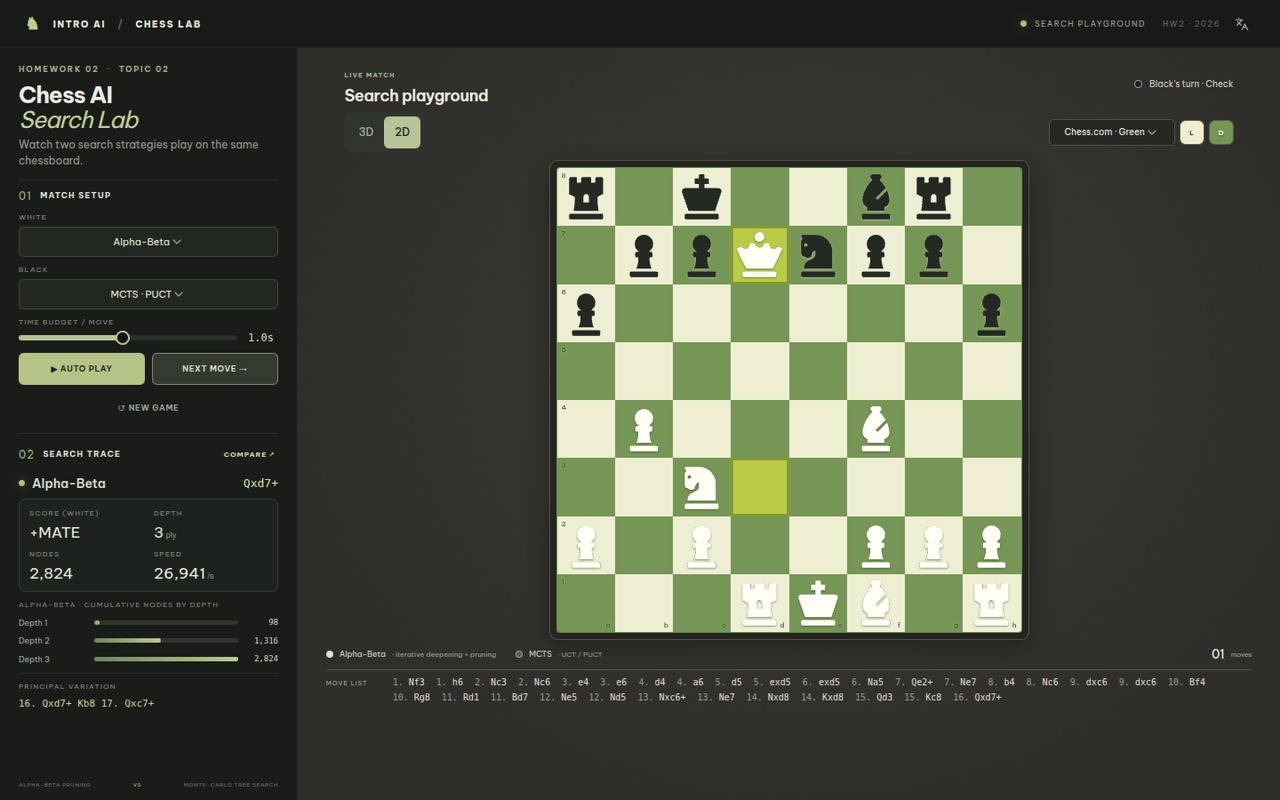
\includegraphics[width=7.85cm]{images/lab_trap_ab.jpg}};
      % 2x Zoom Loupe anchored cleanly at bottom-right over board margins
      \node[anchor=south east, inner sep=2pt, draw=HudTeal, line width=1.1pt,
            fill=HudBgDeep, rounded corners=4pt] (loupe) at (8.02,0.08)
        {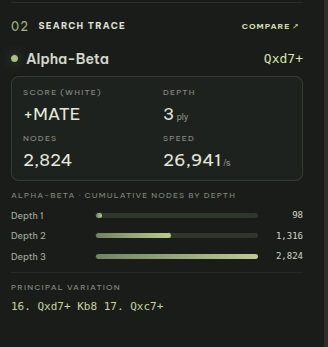
\includegraphics[width=2.68cm]{images/lab_trap_ab_zoom.jpg}};
      \node[anchor=south east, fill=HudBgDeep, draw=HudTeal, line width=0.6pt,
            rounded corners=2pt, inner xsep=4pt, inner ysep=1.5pt,
            font=\ttfamily\fontsize{5.8}{6.8}\selectfont\bfseries, text=HudTeal]
        at ($(loupe.north east)+(-0.06,-0.02)$) {ZOOM $\cdot$ AB TRACE};
      % Connector from trace panel to loupe
      \draw[HudTeal, line width=0.9pt, dashed, -{Stealth[length=1.8mm]}]
        (1.80,1.30) -- (loupe.west);
    \end{tikzpicture}
  \end{column}
  \begin{column}{5.60cm}
    \hudcardaccent[5.5pt]{HudLavender}{4.95cm}{%
      {\ttfamily\fontsize{6.8}{8}\selectfont\bfseries\color{HudLavender}ALPHA-BETA (SEARCH LAB)}\\[1.5pt]
      {\huddisplay\fontsize{14.5}{16.5}\selectfont\color{HudIvory}Qxd7+}\\[1.5pt]
      {\fontsize{7.8}{10.5}\selectfont\color{HudTeal}Proves forced mate $\cdot$ depth 3 $\cdot$ 2,824 nodes}%
    }\par\vspace{5pt}
    \hudcardaccent[5.5pt]{HudCrimson}{4.95cm}{%
      {\ttfamily\fontsize{6.8}{8}\selectfont\bfseries\color{HudGold}MCTS-EVAL (COMPARE)}\\[1.5pt]
      {\huddisplay\fontsize{14.5}{16.5}\selectfont\color{HudIvory}Nd5}\\[1.5pt]
      {\fontsize{7.8}{10.5}\selectfont\color{HudCrimson}Misses mate $\cdot$ deepest path 18 $\cdot$ 33,756 nodes}%
    }\par\vspace{5pt}
    \hudcardaccent[5.5pt]{HudGold}{4.95cm}{%
      {\ttfamily\fontsize{6.6}{7.8}\selectfont\bfseries\color{HudGold}CHRONICLE $\cdot$ FORCED MATE}\\[2pt]
      {\ttfamily\fontsize{7.0}{9}\selectfont\color{HudIvory}16. Qxd7+ Kb8 \ 17. Qxc7+ Ka7 \ 18. Be3\#}%
    }
  \end{column}
\end{columns}
\end{frame}

% SLIDE 11 — LIMITATIONS AND NEXT STEPS (Unified Dark Theme + Paired Status Cards!)
\begin{frame}{LIMITATIONS AND NEXT STEPS}
\hudslidetag[HudGold]{HONEST ASSESSMENT}
\framesubtitle{The conclusion is specific to these agents, datasets, and small time budgets}
\vspace{0.08cm}

\noindent\begin{tikzpicture}[x=1cm,y=1cm]
  \useasboundingbox (0,0.48) rectangle (14.3,4.45);
  \hudlimpair{3.95}{Small sample sizes (8 games/pair, 18--20 traps)}{Expand openings, games, and random seeds}
  \hudlimpair{2.96}{Shallow tactical labels ($\le$ mate in 2)}{Test deeper independently verified suites}
  \hudlimpair{1.97}{Wall-clock budgets \& CPU load noise}{Repeat experiments under fixed node budgets}
  \hudlimpair{0.98}{Handcrafted eval; MCTS resets tree per move}{Add learned policy/value nets \& MCTS tree reuse}
\end{tikzpicture}\par
\vspace{0.06cm}
\hudcardaccent[6pt]{HudGold}{13.55cm}{%
  {\fontsize{8.1}{10.5}\selectfont\color{HudMuted}\textbf{\color{HudGold}E2 saturation:} Alpha-Beta scored 94--100\% across 0.05--1.6\,s; scaling needs a handicap budget test.}%
}
\end{frame}

% SLIDE 12 — CONCLUSIONS (Metric Parallelism: 48/48 | 191x | 0/18)
\begin{frame}{CONCLUSIONS}
\hudslidetag[HudLavender]{MAIN TAKEAWAYS}
\framesubtitle{Under a shared handcrafted evaluation and small search budgets}
\vspace{0.15cm}
\begin{columns}[T,onlytextwidth]
  \begin{column}{4.55cm}
    \hudcard[inner sep=8pt]{3.95cm}{%
      \hudhero[HudLavender]{28}{48/48}\\[5pt]
      {\fontsize{9.2}{11.5}\selectfont\bfseries\color{HudIvory}Observed Tournament Wins}\\[3pt]
      {\fontsize{7.8}{10.5}\selectfont\color{HudMuted}Alpha-Beta won every game by checkmate across 6 opponents}\\[7pt]
      {\tikz\draw[HudLavender, line width=1.6pt] (0,0) -- (3.6,0);}%
    }
  \end{column}
  \begin{column}{4.55cm}
    \hudcard[inner sep=8pt]{3.95cm}{%
      \hudhero[HudGold]{28}{191\textsf{\fontsize{20}{20}\selectfont$\times$}}\\[5pt]
      {\fontsize{9.2}{11.5}\selectfont\bfseries\color{HudIvory}Fewer Nodes at Depth 4}\\[3pt]
      {\fontsize{7.8}{10.5}\selectfont\color{HudMuted}Move ordering + TT vs plain Minimax ($b^*\!: 35 \to 9.4$)}\\[7pt]
      {\tikz\draw[HudGold, line width=1.6pt] (0,0) -- (3.6,0);}%
    }
  \end{column}
  \begin{column}{4.55cm}
    \hudcard[inner sep=8pt]{3.95cm}{%
      \hudhero[HudTeal]{28}{0/18}\\[5pt]
      {\fontsize{9.2}{11.5}\selectfont\bfseries\color{HudIvory}Trap Blunders (Hybrid-d2)}\\[3pt]
      {\fontsize{7.8}{10.5}\selectfont\color{HudMuted}Eliminated traps, but leaf probes cut score from 73\% to 34\%}\\[7pt]
      {\tikz\draw[HudTeal, line width=1.6pt] (0,0) -- (3.6,0);}%
    }
  \end{column}
\end{columns}\par
\vspace{0.20cm}
\hudcardaccent[6.5pt]{HudBorder}{13.55cm}{%
  {\centering\fontsize{8.5}{11}\selectfont\color{HudIvory}With shared evaluation and small budgets, Alpha-Beta outperformed the tested MCTS variants.\par}%
}\par
\vspace{0.22cm}
\noindent\begin{minipage}{\textwidth}
  {\huddisplay\fontsize{16}{19}\selectfont\color{HudGold}QUESTIONS?}
  \hfill
  {\ttfamily\fontsize{8}{10}\selectfont\color{HudLavender}\href{https://github.com/HatakekkSheeshh/hw2_introAI}{github.com/HatakekkSheeshh/hw2\_introAI}}
\end{minipage}
\end{frame}

% ======================================================================
% APPENDIX — Q&A BACKUP SLIDES (Q1–Q6)
% ======================================================================
\hudstartappendix

% Q1 — ALPHA-BETA: IMPLEMENTATION
\begin{frame}{ALPHA-BETA: IMPLEMENTATION}
\hudslidetag[HudLavender]{Q\&A BACKUP $\cdot$ Q1}
\framesubtitle{Distinguishing exact pruning from selective search heuristics}
\vspace{0.12cm}
\begin{columns}[T,onlytextwidth]
  \begin{column}{6.85cm}
    \hudcardaccent[8pt]{HudLavender}{6.20cm}{%
      {\ttfamily\fontsize{7.4}{8.8}\selectfont\bfseries\color{HudLavender}EXACT PRUNING (MINIMAX-EQUIVALENT)}\\[5pt]
      {\fontsize{8.3}{12.5}\selectfont\color{HudIvory}%
        \hudcheck\ \ Negamax formulation with $\alpha$--$\beta$ bounds\\
        \hudcheck\ \ Transposition table (exact / lower / upper flags)\\
        \hudcheck\ \ Iterative deepening (reuses PV across plies)\\
        \hudcheck\ \ Move ordering: TT move, MVV-LVA, killer, history%
      }%
    }
  \end{column}
  \begin{column}{6.85cm}
    \hudcardaccent[8pt]{HudTeal}{6.20cm}{%
      {\ttfamily\fontsize{7.4}{8.8}\selectfont\bfseries\color{HudTeal}SELECTIVE EXTENSIONS \& REDUCTIONS}\\[5pt]
      {\fontsize{8.3}{12.5}\selectfont\color{HudIvory}%
        $\bullet$ \textbf{Quiescence search:} resolves captures \& checks at horizon\\
        $\bullet$ \textbf{Null-move pruning:} skips quiet lines on strong fail-high\\
        $\bullet$ \textbf{Late-move reductions (LMR):} searches late quiet moves 1 ply shallower%
      }%
    }
  \end{column}
\end{columns}\par
\vspace{0.18cm}
\hudcardaccent[7pt]{HudGold}{13.55cm}{%
  {\fontsize{8.3}{11.5}\selectfont\color{HudIvory}\textbf{\color{HudGold}Exactness note:} Standard $\alpha$--$\beta$ (AB-Plain, AB-Ordered) preserves Minimax's exact score; AB-Selective ($b^* = 5.9$) trades strict exactness for extra depth.}%
}
\end{frame}

% Q2 — UCT, PUCT AND LEAF VALUES
\begin{frame}{UCT, PUCT AND LEAF EVALUATION}
\hudslidetag[HudGold]{Q\&A BACKUP $\cdot$ Q2}
\framesubtitle{Selection policies, heuristic priors, and value perspective mapping}
\vspace{0.10cm}
\begin{columns}[T,onlytextwidth]
  \begin{column}{6.85cm}
    \hudcardaccent[7.5pt]{HudGold}{6.20cm}{%
      {\ttfamily\fontsize{7.4}{8.8}\selectfont\bfseries\color{HudGold}TREE SELECTION POLICIES}\\[5pt]
      {\fontsize{8.3}{11.5}\selectfont\color{HudIvory}%
        \textbf{MCTS-Random (UCT):}
        \[
          \mathrm{score}(s,a) = Q(s,a) + c \sqrt{\frac{\ln N(s)}{n(s,a)}}
        \]
        \textbf{MCTS-Eval / Solver / Hybrid (PUCT):}
        \[
          \mathrm{score}(s,a) = Q(s,a) + c_{\mathrm{puct}}\, P(s,a)\,\frac{\sqrt{N(s)}}{1 + n(s,a)}
        \]
        {\fontsize{7.6}{10}\selectfont\color{HudMuted}Priors $P(s,a)$ come from handcrafted move-ordering heuristics (not a neural policy network).}%
      }%
    }
  \end{column}
  \begin{column}{6.85cm}
    \hudcardaccent[7.5pt]{HudTeal}{6.20cm}{%
      {\ttfamily\fontsize{7.4}{8.8}\selectfont\bfseries\color{HudTeal}CENTIPAWN MAPPING \& BACKUP}\\[5pt]
      {\fontsize{8.3}{11.5}\selectfont\color{HudIvory}%
        Shared evaluator returns centipawns ($\mathrm{cp}$), mapped to $[-1, 1]$ via:
        \[
          v = \tanh\!\left(\frac{\mathrm{cp}}{400}\right)
        \]
        \textbf{Perspective:} Scores are negated at every ply during backpropagation so parent nodes track side-to-move value.\\[4pt]
        \textbf{Hybrids:} Replace simple leaf evaluation with depth-1 or depth-2 $\alpha$--$\beta$ probes.%
      }%
    }
  \end{column}
\end{columns}
\end{frame}

% Q3 — E2: BUDGET SCALING
\begin{frame}{E2: BUDGET SCALING (0.05\,s -- 1.6\,s)}
\hudslidetag[HudLavender]{Q\&A BACKUP $\cdot$ Q3}
\framesubtitle{Alpha-Beta vs MCTS-Eval across a $32\times$ time-budget range (8 games per budget)}
\vspace{0.10cm}
\hudcard[inner sep=7pt]{13.55cm}{%
  \renewcommand{\arraystretch}{1.18}%
  \fontsize{8.2}{10}\selectfont
  \begin{tabular}{@{}>{\ttfamily\bfseries\color{HudGold}}lccccc@{}}
    \toprule
    \textbf{\color{HudMuted}Time/move} & \textbf{\color{HudMuted}W / D / L (AB)} & \textbf{\color{HudMuted}AB Score} & \textbf{\color{HudMuted}95\% CI} & \textbf{\color{HudMuted}Mean Depth AB} & \textbf{\color{HudMuted}Deepest Path Eval} \\
    \midrule
    0.05\,s & 8 / 0 / 0 & \color{HudLavender}\textbf{100\%} & 68--100\% & 1.9 & 11.4 \\
    0.10\,s & 8 / 0 / 0 & \color{HudLavender}\textbf{100\%} & 68--100\% & 2.5 & 13.4 \\
    0.20\,s & 7 / 1 / 0 & \color{HudLavender}\textbf{94\%}  & 60--99\%  & 3.1 & 14.9 \\
    0.40\,s & 8 / 0 / 0 & \color{HudLavender}\textbf{100\%} & 68--100\% & 3.7 & 16.3 \\
    0.80\,s & 7 / 1 / 0 & \color{HudLavender}\textbf{94\%}  & 60--99\%  & 4.7 & 16.3 \\
    1.60\,s & 8 / 0 / 0 & \color{HudLavender}\textbf{100\%} & 68--100\% & 5.0 & 17.7 \\
    \bottomrule
  \end{tabular}%
}\par
\vspace{0.16cm}
\hudcardaccent[7pt]{HudGold}{13.55cm}{%
  {\fontsize{8.2}{11.2}\selectfont\color{HudIvory}%
    \textbf{\color{HudGold}Saturation caveat:} 46 W / 2 D / 0 L across 48 games ($+0.65$ vs $+1.20$ plies per budget doubling). Because score sits at 94--100\%, this test cannot determine whether MCTS would catch up with much larger budgets.%
  }%
}
\end{frame}

% Q4 — E5: MASTER-MOVE AGREEMENT
\begin{frame}{E5: AGREEMENT WITH MASTER MOVES}
\hudslidetag[HudTeal]{Q\&A BACKUP $\cdot$ Q4}
\framesubtitle{200 middlegame positions from master games (mean rating 2521 $\cdot$ 1.0\,s/move $\cdot$ random chance 2.8\%)}
\vspace{0.10cm}
\begin{columns}[T,onlytextwidth]
  \begin{column}{8.65cm}
    \hudcard[inner sep=9pt]{7.95cm}{%
      \hudbar{Alpha-Beta}{2.15}{3.10}{0.91}{36.5\% \ (73/200)}{HudLavender}\\[8pt]
      \hudbar{MCTS-Solver}{2.15}{3.10}{0.54}{21.5\% \ (43/200)}{HudGold}\\[8pt]
      \hudbar{MCTS-Eval}{2.15}{3.10}{0.53}{21.0\% \ (42/200)}{HudGold}\\[8pt]
      \hudbar{Hybrid-d1}{2.15}{3.10}{0.40}{16.0\% \ (32/200)}{HudTeal}\\[8pt]
      \hudbar{Random}{2.15}{3.10}{0.13}{5.0\% \ \ (10/200)}{HudStone}\\[8pt]
      \hudbar{MCTS-Random}{2.15}{3.10}{0.11}{4.5\% \ \ (9/200)}{HudMuted}
    }
  \end{column}
  \begin{column}{5.25cm}
    \hudcardaccent[7.5pt]{HudLavender}{4.65cm}{%
      {\ttfamily\fontsize{7}{8}\selectfont\bfseries\color{HudLavender}KEY METRICS AT 1.0\,s}\\[5pt]
      {\fontsize{8.2}{11.8}\selectfont\color{HudIvory}%
        $\bullet$ AB $\kappa = \mathbf{0.35}$ vs Solver/Eval $\kappa = \mathbf{0.19}$\\
        $\bullet$ Spearman correlation with E1 Elo: $\boldsymbol{\rho = 0.89}$%
      }%
    }\par\vspace{8pt}
    \hudcardaccent[7.5pt]{HudGold}{4.65cm}{%
      {\ttfamily\fontsize{7}{8}\selectfont\bfseries\color{HudGold}INTERPRETATION CAVEAT}\\[5pt]
      {\fontsize{8.1}{11.2}\selectfont\color{HudMuted}Master moves are not unique ground truth; agreement is a coarse non-tactical proxy rather than absolute accuracy.}%
    }
  \end{column}
\end{columns}
\end{frame}

% Q5 — REPRODUCIBILITY AND FAIRNESS
\begin{frame}{REPRODUCIBILITY AND FAIRNESS}
\hudslidetag[HudGold]{Q\&A BACKUP $\cdot$ Q5}
\framesubtitle{Experimental controls and explicit asymmetries in the benchmark}
\vspace{0.12cm}
\begin{columns}[T,onlytextwidth]
  \begin{column}{6.85cm}
    \hudcardaccent[8pt]{HudTeal}{6.20cm}{%
      {\ttfamily\fontsize{7.4}{8.8}\selectfont\bfseries\color{HudTeal}CONTROLLED PROTOCOL}\\[5pt]
      {\fontsize{8.3}{12}\selectfont\color{HudIvory}%
        \hudcheck\ \ \textbf{Shared evaluator:} identical material + PSTs for AB \& MCTS-Eval\\
        \hudcheck\ \ \textbf{Balanced colours:} 4 openings $\times$ both sides (77 White, 82 Black, 9 draws)\\
        \hudcheck\ \ \textbf{Deterministic seed:} \texttt{seed = 42}, shared symmetric adjudication at 120 plies\\
        \hudcheck\ \ \textbf{Similar work:} 22k--30k nodes/move across searching agents%
      }%
    }
  \end{column}
  \begin{column}{6.85cm}
    \hudcardaccent[8pt]{HudGold}{6.20cm}{%
      {\ttfamily\fontsize{7.4}{8.8}\selectfont\bfseries\color{HudGold}REPORTED ASYMMETRIES}\\[5pt]
      {\fontsize{8.3}{12}\selectfont\color{HudIvory}%
        $\bullet$ \textbf{Memory:} Alpha-Beta retains its transposition table across moves; MCTS rebuilds from root each turn\\
        $\bullet$ \textbf{Time noise:} wall-clock 1\,s budgets vary slightly with CPU load\\
        $\bullet$ \textbf{Elo scale:} relative Bradley--Terry fit (Random = 0, virtual-draw prior), \textit{not} FIDE Elo%
      }%
    }
  \end{column}
\end{columns}
\end{frame}

% Q6 — GROUP 7 TEAM & REFERENCES (Vietnamese Unicode in Inter!)
\begin{frame}{GROUP 7 $\cdot$ CC01 — TEAM \& REFERENCES}
\hudslidetag[HudLavender]{Q\&A BACKUP $\cdot$ Q6}
\framesubtitle{CO3061 Introduction to Artificial Intelligence $\cdot$ Advisor: Dr. Nguyễn Quốc Minh}
\vspace{0.04cm}
\begin{columns}[T,onlytextwidth]
  \begin{column}{8.9cm}
    \hudcard[inner sep=5pt]{8.35cm}{%
      \setlength{\tabcolsep}{4pt}%
      \renewcommand{\arraystretch}{1.04}%
      \fontsize{7.0}{8.4}\selectfont
      \begin{tabular}{@{}>{\color{HudIvory}}p{2.45cm}>{\ttfamily\color{HudLavender}}p{1.05cm}>{\color{HudMuted}}p{4.20cm}@{}}
        \toprule
        \textbf{\color{HudGold}Member} & \textbf{\color{HudGold}ID} & \textbf{\color{HudGold}Primary Contribution} \\
        \midrule
        Nguyễn Quốc Hiệu & 2352344 & Search agents, hybrids \& E1--E5 \\
        Quách Hoàng Phú & 2352922 & Evaluation, arena \& background \\
        Chu Nguyễn Tuấn Anh & 2352022 & Search Lab UI, CI \& LaTeX setup \\
        Lê Hoàng Chí Vĩ & 2353336 & Datasets, mate solver \& labels \\
        Vũ Hải Tuấn & 2353280 & Statistics, Wilson CIs, Elo \& plots \\
        Nguyễn Lê Đăng Vinh & 2353330 & GUI case study, MCTS trace \& report \\
        Dương Nguyễn Tấn Đạt & 2352222 & Python web UI, API \& i18n \\
        Đỗ Thái Phong & 2352903 & Unit tests, discussion \& conclusions \\
        \bottomrule
      \end{tabular}%
    }
  \end{column}
  \begin{column}{4.95cm}
    \hudcardaccent[6.5pt]{HudGold}{4.45cm}{%
      {\ttfamily\fontsize{6.8}{7.8}\selectfont\bfseries\color{HudGold}KEY REFERENCES}\\[4pt]
      {\fontsize{7.3}{9.8}\selectfont\color{HudMuted}%
        $\bullet$ Knuth \& Moore (1975): \textit{An analysis of alpha-beta pruning}\\
        $\bullet$ Ramanujan et al. (2010): \textit{Adversarial planning \& search traps}\\
        $\bullet$ Silver et al. (2018): \textit{AlphaZero (Science)}\\
        $\bullet$ Baier \& Winands (2018): \textit{MCTS-Minimax hybrids}%
      }%
    }\par\vspace{6pt}
    \hudcard[inner sep=6pt]{4.45cm}{%
      \centering
      
\includegraphics[height=0.58cm]{images/BK.png}\\[3pt]
      {\fontsize{7.3}{9}\selectfont\color{HudIvory}HCMUT $\cdot$ VNU-HCM}\\
      {\ttfamily\fontsize{6.4}{7.8}\selectfont\color{HudTeal}\href{https://github.com/HatakekkSheeshh/hw2_introAI}{HatakekkSheeshh/hw2\_introAI}}%
    }
  \end{column}
\end{columns}
\end{frame}

\end{document}
